\documentclass{article}
\usepackage[utf8]{inputenc}
\usepackage{geometry}
\usepackage{url}
\usepackage[utopia]{mathdesign}
\usepackage{amsmath}
 \geometry{
 a4paper,
 total={170mm,257mm},
 left=20mm,
 top=20mm,
 }
\usepackage{graphicx}
\usepackage{tikz}
\usepackage{titling}
\usepackage{kinematikz}
 \title{1st report of Advanced Topics in Robot Mechanism
}
\author{GU JUN}
\date{Nov 18. 2024}
 
 \usepackage{fancyhdr}
\fancypagestyle{plain}{%  the preset of fancyhdr 
    \fancyhf{} % clear all header and footer fields
    \fancyfoot[R]{\thepage}
    \fancyfoot[L]{\theauthor}
    \fancyhead[L]{2024 Advanced Topics in Robot Mechanism}
    \fancyhead[R]{\thedate}
}
\makeatletter
\def\@maketitle{%
  \newpage
  \null
  \vskip 1em%
  \begin{center}%
  \let \footnote \thanks
    {\LARGE \@title \par}%
    \vskip 1em%
    %{\large \@date}%
  \end{center}%
  \par
  \vskip 1em}
\makeatother

\usepackage{lipsum}  
\usepackage{cmbright}

\begin{document}

\maketitle

\noindent\begin{tabular}{@{}ll}
    Student & \theauthor\\
    Student ID & 61322300564 \\
    Date & \thedate\\
\end{tabular}

\section*{A manipulator with 4 DOF}

The manipulator consists of 4 degrees of freedom (DOF) with 3 revolute joints and 1 prismatic joint. 
The manipulator is shown in Fig.\ref{fig:manipulator_4dof}. For this manipulator, the base frame is denoted as R, and the end-effector frame is denoted as E. 
The joints are labeled as J1, J2, J3, and J4.
When the joint variables are set to specific values, the manipulator can be configured in different positions and orientations in 3D space.

\begin{figure}[h!]
\centering
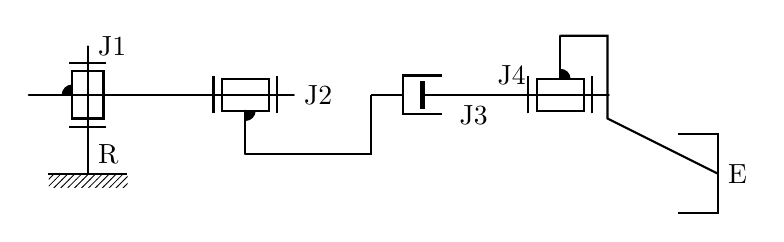
\begin{tikzpicture}[knLinkStyle,node distance=1cm and 2cm]
\pic (J0) {frame} node [above right] {R};
\pic [rotate=90](J1) [above=of J0-out] {revolute pair spatial=90:0.75/0/0};
\node [anchor=west,at=(J1-in2)] {J1};
\pic  (J2) [right=of J1-center] {revolute pair spatial=-90:0.75/1/0};
\node [anchor=west,at=(J2-in2)] {J2};
\pic  (J3) [right=of J2-center] {linear piston = 0.5};
\node [anchor=north,at=(J3-out)] {J3};
\pic (J4) [right=of J3-center] {revolute pair spatial=90:0.75/0/0};
\node [anchor=south,at=(J4-in)] {J4};
\pic (GR) [rotate=180][below right=of J4-center] {gripper};
\node [anchor=west,at=(GR-in)] {E};
\draw [] (J0-out) -- ($(J0-out)!0.5!(J1-center)$) -| (J1-in);
\draw [] (J1-out) -| (J2-in);
\draw [] (J2-out) -| (J3-in);
\draw [] (J3-out) -| (J4-in);
\draw [] (J4-out) -| ($(J4-center)!0.3!(GR-in)$) -- (GR-in);
\end{tikzpicture}
\caption{Manipulator with 4 DOF, 3 revolute joints and 1 prismatic joint}
\label{fig:manipulator_4dof}
\end{figure}


\section*{DH Notation for Structure Definition}

\begin{figure}[h!]
  \centering
  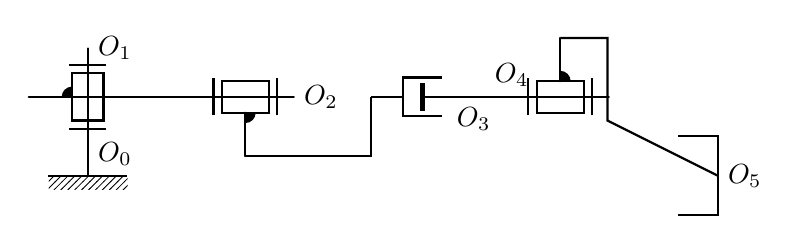
\begin{tikzpicture}[knLinkStyle,node distance=1cm and 2cm]
    \pic (J0) {frame} node [above right] {$O_0$};
    \pic [rotate=90](J1) [above=of J0-out] {revolute pair spatial=90:0.75/0/0};
    \node [anchor=west,at=(J1-in2)] {$O_1$};
    \pic  (J2) [right=of J1-center] {revolute pair spatial=-90:0.75/1/0};
    \node [anchor=west,at=(J2-in2)] {$O_2$};
    \pic  (J3) [right=of J2-center] {linear piston = 0.5};
    \node [anchor=north,at=(J3-out)] {$O_3$};
    \pic (J4) [right=of J3-center] {revolute pair spatial=90:0.75/0/0};
    \node [anchor=south,at=(J4-in)] {$O_4$};
    \pic (GR) [rotate=180][below right=of J4-center] {gripper};
    \node [anchor=west,at=(GR-in)] {$O_5$};
    \draw [] (J0-out) -- ($(J0-out)!0.5!(J1-center)$) -| (J1-in);
    \draw [] (J1-out) -| (J2-in);
    \draw [] (J2-out) -| (J3-in);
    \draw [] (J3-out) -| (J4-in);
    \draw [] (J4-out) -| ($(J4-center)!0.3!(GR-in)$) -- (GR-in);
    \end{tikzpicture}
    \caption{Define the coordinates of the manipulator}
      \label{fig:manipulator_4dofwithlabel}
  \end{figure}

After define the coordinates of the manipulator, we can use the DH parameters to define the structure of the manipulator.
All lengths and angles are given with a set value. The DH parameters for the manipulator are shown in Table.\ref{tab:dh_parameters}.
\begin{table}[h!]
  \centering
  \begin{tabular}{|c|c|c|c|c|}
  \hline
  Joint & $a_{i-1}$ & $\alpha_{i-1}$ & $d_i$ & $\theta_i$ \\
  \hline
  1 & $0$ & $0$ & $1$ & $\theta_1$ \\
  2 & $1$ & $\frac{\pi}{2}$ & $0$ & $\theta_2$ \\
  3 & $1$ & $0$ & $d_3$ & $0$ \\
  4 & $0$ & $0$ & $0$ & $\theta_4$ \\
  5 & $0$ & $-\pi$ & $0.1$ & $0$ \\
  \hline
  \end{tabular}
  \caption{DH Parameters for a 3 DOF Robot Arm}
  \label{tab:dh_parameters}
\end{table}
  
\section*{Kinematic Equation Derivation}
The transformation matrix for each joint using DH parameters is given by:

\begin{equation}
  { }^{n-1} T_n=\left[\begin{array}{ccc|c}
  \cos \theta_n & -\sin \theta_n & 0 & a_{n-1} \\
  \sin \theta_n \cos \alpha_{n-1} & \cos \theta_n \cos \alpha_{n-1} & -\sin \alpha_{n-1} & -d_n \sin \alpha_{n-1} \\
  \sin \theta_n \sin \alpha_{n-1} & \cos \theta_n \sin \alpha_{n-1} & \cos \alpha_{n-1} & d_n \cos \alpha_{n-1} \\
  \hline 0 & 0 & 0 & 1
  \end{array}\right]
  \end{equation}
  
For the given manipulator, the overall transformation matrix from the base to the end-effector is the product of the individual transformation matrices:

\[
T = T_1 \cdot T_2 \cdot T_3 \cdot T_4
\]

Where each \(T_i\) is calculated using the corresponding DH parameters.

Given the DH parameters, we can calculate the transformation matrices for each joint:

\[
T_1 = 
\begin{bmatrix}
\cos(\theta_1) & -\sin(\theta_1) & 0 & 0 \\
\sin(\theta_1) & \cos(\theta_1) & 0 & 0 \\
0 & 0 & 1 & 1 \\
0 & 0 & 0 & 1
\end{bmatrix}
\quad
T_2 = 
\begin{bmatrix}
\cos(\theta_2) & -\sin(\theta_2) & 0 & 1 \\
0 & 0 & -1 & 0 \\
\sin(\theta_2) & \cos(\theta_2) & 0 & 0 \\
0 & 0 & 0 & 1
\end{bmatrix}
\]


\[
T_3 = \begin{bmatrix}
1 & 0 & 0 & 1 \\
0 & 1 & 0 & 0 \\
0 & 0 & 1 & d_3 \\
0 & 0 & 0 & 1
\end{bmatrix}
\quad
T_4 = \begin{bmatrix}
\cos(\theta_4) & -\sin(\theta_4) & 0 & 0 \\
\sin(\theta_4) & \cos(\theta_4)  & 0 & 0 \\
0 & 0 & 1 & 0 \\
0 & 0 & 0 & 1
\end{bmatrix}
\quad
T_5 = \begin{bmatrix}
1 & 0 & 0 & 0 \\
0 & -1  & 0 & 0 \\
0 & 0 & -1 & -0.1 \\
0 & 0 & 0 & 1
\end{bmatrix}
\]


The overall transformation matrix \( T \) is:

\[
T = T_1 \cdot T_2 \cdot T_3 \cdot T_4 \cdot T_5
\]

Calculating the product:

\[
T = \begin{bmatrix}
\cos(\theta_1) & -\sin(\theta_1) & 0 & 0 \\
\sin(\theta_1) & \cos(\theta_1) & 0 & 0 \\
0 & 0 & 1 & 1 \\
0 & 0 & 0 & 1
\end{bmatrix}
\cdot
\begin{bmatrix}
\cos(\theta_2) & -\sin(\theta_2) & 0 & 1 \\
0 & 0 & -1 & 0 \\
\sin(\theta_2) & \cos(\theta_2) & 0 & 0 \\
0 & 0 & 0 & 1
\end{bmatrix}
\]

\[
\cdot
\begin{bmatrix}
1 & 0 & 0 & 1 \\
0 & 1 & 0 & 0 \\
0 & 0 & 1 & d_3 \\
0 & 0 & 0 & 1
\end{bmatrix}
\cdot
\begin{bmatrix}
\cos(\theta_4) & -\sin(\theta_4) & 0 & 0 \\
\sin(\theta_4) & \cos(\theta_4)  & 0 & 0 \\
0 & 0 & 1 & 0 \\
0 & 0 & 0 & 1
\end{bmatrix}
\cdot
\begin{bmatrix}
1 & 0 & 0 & 0 \\
0 & -1  & 0 & 0 \\
0 & 0 & -1 & -0.1 \\
0 & 0 & 0 & 1
\end{bmatrix}
\]

\[
T = \begin{bmatrix}
c_1 c_2 c_4 - c_1 s_2 s_4 & c_1 c_2 s_4 + c_1 c_4 s_2 & -s_1 & c_1 - \frac{s_1}{10} + c_1 c_2 + d_3 s_1 \\
c_2 c_4 s_1 - s_1 s_2 s_4 & c_2 s_1 s_4 + c_4 s_1 s_2 & c_1 & \frac{c_1}{10} + s_1 + c_2 s_1 - d_3 c_1 \\
c_2 s_4 + c_4 s_2 & s_2 s_4 - c_2 c_4 & 0 & s_2 + 1 \\
0 & 0 & 0 & 1
\end{bmatrix}
\]

The above matrix \( T \) represents the overall transformation matrix from the base to the end-effector of the manipulator. Here, $c_i$ and $s_i$ are shorthand notations for $\cos(\theta_i)$  and  $\sin(\theta_i) $ respectively. This matrix is derived by multiplying the individual transformation matrices \( T_1, T_2, T_3, T_4, \) and \( T_5 \) using the given DH parameters.

With this matrix, we can calculate the endpoint position and posture of the manipulator for different joint variables.
\section*{Joint Variables and Endpoint Positions Calculation}

To verify the correctness of the derived kinematic equation, we calculate the endpoint positions for different joint variables. The following table shows the joint variables and their corresponding endpoint positions:

\begin{table}[h!]
  \centering
  \begin{tabular}{|c|c|c|c|}
  \hline
  $\theta_1$ & $\theta_2$ & $d_3$ & $\theta_4$ \\
  \hline
  $0$ & $0$ & $0.5$ & 0 \\
  $\frac{\pi}{4}$ & $\frac{\pi}{4}$ & $1$ & $\frac{\pi}{4}$\\
  $\frac{\pi}{2}$ & $\frac{\pi}{2}$ & $1.5$ & $0$\\
  \hline
  \end{tabular}
  \caption{Joint Variables for testing}
  \label{tab:joint_variables}
\end{table}

Using these joint variables, we calculate the transformation matrix
\( T \) and extract the endpoint position from the matrix.\\
For the joint variables \(\theta_1 = 0\), \(\theta_2 = 0\), \(d_3 = 0.5\), and \(\theta_4 = 0\),
the transformation matrix \( T \) is:

\[
T = \begin{bmatrix}
1 & 0 & 0 & 2 \\
0 & 0 & 1 & -0.4 \\
0 & -1 & 0 & 1 \\
0 & 0 & 0 & 1
\end{bmatrix}
\]

For the joint variables \(\theta_1 = \frac{\pi}{4}\), \(\theta_2 = \frac{\pi}{4}\), \(d_3 = 1\), and \(\theta_4 = \frac{\pi}{4}\),
the transformation matrix \( T \) is:

\[
T = \begin{bmatrix}
0 & \frac{\sqrt{2}}{2} & -\frac{\sqrt{2}}{2} & \frac{19\sqrt{2}}{20} + \frac{1}{2} \\
0 & \frac{\sqrt{2}}{2} & \frac{\sqrt{2}}{2} & \frac{\sqrt{2}}{20} + \frac{1}{2} \\
1 & 0 & 0 & \frac{\sqrt{2}}{2} + 1 \\
0 & 0 & 0 & 1
\end{bmatrix}
\]


For the joint variables \(\theta_1 = \frac{\pi}{2}\), \(\theta_2 = \frac{\pi}{2}\), \(d_3 = 1.5\), and \(\theta_4 = 0\),
the transformation matrix \( T \) is:

\[
T = \begin{bmatrix}
0 & 0 & -1 & \frac{7}{5} \\
0 & 1 & 0 & 1 \\
1 & 0 & 0 & 2 \\
0 & 0 & 0 & 1
\end{bmatrix}
\]

The last column of each matrix represents the endpoint position of the manipulator for the given 
joint variables. 
The calculated endpoint positions are shown in the following table(after rounding off to 4 decimal places):

\begin{table}[h!]
  \centering
  \begin{tabular}{|c|c|c|c|c|}
  \hline
  $\theta_1$ & $\theta_2$ & $d_3$ & $\theta_4$ & Endpoint Position $(x, y, z)$ \\
  \hline
  $0$ & $0$ & $0.5$ & 0 & $(2, -0.4, 1)$ \\
  $\frac{\pi}{4}$ & $\frac{\pi}{4}$ & $1$ & $\frac{\pi}{4}$ & $(1.8435, 0.5707, 1.7071)$ \\
  $\frac{\pi}{2}$ & $\frac{\pi}{2}$ & $1.5$ & $0$ & $(1.4, 1, 2)$ \\
  \hline
  \end{tabular}
  \caption{Joint Variables and Corresponding Endpoint Positions}
  \label{tab:endpoint_positions}
\end{table}

\section*{Matlab simulation \& Verification of the manipulator}

I use Matlab rigid body tree to prove my result. The main process is define the rigid body tree, 
set the joint variables, and get the endpoint position. 
Then compare the result with the calculated result to verify the correctness of the kinematic equation. 

\subsection*{Modeling Using DH Parameters}
To verify the calculated results, I modeled the manipulator using the DH parameters in Matlab. 
The manipulator is modeled as a rigid body tree with 5 joints and 5 links.
The DH parameters are used to define the structure of the manipulator.
One thing to note is that there are 'dh' and 'mdh' options in the rigid body tree.
The 'dh' option uses the Denavit-Hartenberg convention for the joint transformations, 
while the 'mdh' option uses the modified Denavit-Hartenberg convention.
In our case, we need to use the 'mdh' option to define the manipulator structure.
With the DH parameters from table.\ref{tab:dh_parameters}, we can define the rigid body tree for the manipulator as follows:
\begin{figure}[h]
  \centering
  \includegraphics[width=0.4\textwidth]{a_simple_3_dof_robot_arm.pdf}
  \caption{The 4 DOF Robot Arm Model, all joint variables are set to zero}
  \label{fig:simple_3_dof_robot_arm}
\end{figure}

With the joint variables as table.\ref{tab:joint_variables}, we can get the endpoint position of the manipulator.
The endpoint positions are calculated using the forward kinematics function of the rigid body tree.
And the result is showing in the following figures.
\subsection*{Matlab Result}

\begin{figure}[h!]
  \centering
  \includegraphics[width=0.3\textwidth]{configuration_1.pdf}
  \caption{Manipulator configuration for $\theta_1 = 0$, $\theta_2 = 0$, $d_3 = 0.5$, $\theta_4 = 0$}
  \label{fig:configuration_1}
\end{figure}

\begin{figure}[h!]
  \centering
  \includegraphics[width=0.3\textwidth]{configuration_2.pdf}
  \caption{Manipulator configuration for $\theta_1 = \frac{\pi}{4}$, $\theta_2 = \frac{\pi}{4}$, $d_3 = 1$, $\theta_4 = \frac{\pi}{4}$}
  \label{fig:configuration_2}
\end{figure}

\begin{figure}[h!]
  \centering
  \includegraphics[width=0.3\textwidth]{configuration_3.pdf}
  \caption{Manipulator configuration for $\theta_1 = \frac{\pi}{2}$, $\theta_2 = \frac{\pi}{2}$, $d_3 = 1.5$, $\theta_4 = 0$}
  \label{fig:configuration_3}
\end{figure}

\begin{table}[h!]
  \centering
  \begin{tabular}{|c|c|c|c|c|c|}
  \hline
  $\theta_1$ & $\theta_2$ & $d_3$ & $\theta_4$ & Endpoint Position $(x, y, z)$ calculated & Endpoint position in Matlab \\
  \hline
  $0$ & $0$ & $0.5$ & 0 & $(2, -0.4, 1)$ & $2.0000, -0.4000, 1.0000$\\
  $\frac{\pi}{4}$ & $\frac{\pi}{4}$ & $1$ & $\frac{\pi}{4}$ & $(1.8435, 0.5707, 1.7071)$ & $(1.8435, 0.5707, 1.7071)$\\
  $\frac{\pi}{2}$ & $\frac{\pi}{2}$ & $1.5$ & $0$ & $(1.4, 1, 2)$ & $(1.4000, 1.0000, 2.0000)$ \\
  \hline
  \end{tabular}
  \caption{Comparison of Calculated and Matlab Endpoint Positions}
  \label{tab:endpoint_positions}
\end{table}

The endpoint positions calculated using the kinematic equation and the endpoint positions obtained from the Matlab simulation are consistent.

\newpage

\section*{Appendix}
\subsection*{Matlab Code}
\begin{verbatim}
% Define DH parameters: [a alpha d theta]
theta1 = 0;
theta2 = 0;
theta3 = 0;
dhparams = [0   	0   	1   	0;
  1	    pi/2       0    0;
  1	    0	    -0.2	0;
  0   	0   	0   	0;
  0       -pi 	0.1   	0;];
% Create a rigid body tree
robot = robotics.RigidBodyTree;
bodies = cell(5,1);
joints = cell(5,1);
for i = 1:5
  bodies{i} = rigidBody(['body' num2str(i)]);
  if i == 3
    joints{i} = rigidBodyJoint(['jnt' num2str(i)],"prismatic");
  else
    joints{i} = rigidBodyJoint(['jnt' num2str(i)],"revolute");
  end
  setFixedTransform(joints{i},dhparams(i,:),"mdh");
  bodies{i}.Joint = joints{i};
  if i == 1 % Add first body to base
    addBody(robot,bodies{i},"base")
  else % Add current body to previous body by name
    addBody(robot,bodies{i},bodies{i-1}.Name)
  end
end
% Define configurations based on the table
configurations = [0, 0, 0.5, 0;
                  pi/4, pi/4, 1, pi/4;
                  pi/2, pi/2, 1.5, 0];
% Loop through each configuration and display the robot
for i = 1:size(configurations, 1)
  config = homeConfiguration(robot);
  config(1).JointPosition = configurations(i, 1);
  config(2).JointPosition = configurations(i, 2);
  config(3).JointPosition = configurations(i, 3);
  config(4).JointPosition = configurations(i, 4);
  % Get the transformation from the base to the end effector  
  tform = getTransform(robot, config, 'body5');
  % Extract the position from the transformation matrix
  position = tform(1:3, 4);
  % Show the robot with the updated configuration
  show(robot, config, 'PreservePlot', false, 'Visuals', 'on');
  % Plot the position of the end effector
  % Display the position of the end effector
  disp(['End effector position for configuration ' num2str(i) ':']);
  disp(position);
  title(['Configuration ' num2str(i)]);
  drawnow;
  pause(1); % Pause to visualize each configuration
end
\end{verbatim}
\end{document}
